\providecommand{\atd}{..}
\documentclass[../ATD.tex]{subfiles}

\begin{document}
    \chapter{Application and document analysis}\label{ch:application-and-document-analysis}
    \section{Application analysis}\label{sec:application-analysis}
    \subsection{Features analysis}\label{subsec:feature-analysis}
    In these section we want to provide a recap of the feature of the system that work correctly, partially work or do not work at all.
    \newline
    \textbf{Working features}
    \begin{itemize}
        \item User log-in
        \item Municipality log-in
    \end{itemize}
    \textbf{Partially working feature}
    \begin{itemize}
        \item Municipality violation query
    \end{itemize}

    \textbf{Not working feature}
    \begin{itemize}
        \item Registration
        \item Violation reporting
        \item Statistics querying
        \item Map visualization
    \end{itemize}
    \subsection{Requirement analysis}\label{subsec:requirement-analysis}
    Here is presented a table to recap which requirements pass the tests and which do not.

    \begin{enumerate}
        \requirement{1} The reports about the violations are correctly stored.
        \requirement{2} The user can view the statistics calculated by the system with some exceptions.
        \requirement{3} The municipality can access only the data of the violations of its competence area.
        \requirement{4} Violations registered by the municipality can be retrieved by the system.
        \requirement{5} The system must avoid the manipulation of the violations.
        \requirement{6} The system must be able to retrieve the position from the user or from the GPS.
        \requirement{7} Only the municipality can access the submitted parking violation of its competence area.
        \requirement{8} The system must allow the user to take a picture or to select one from the device.
        \requirement{9} The system accepts reports from the user.
        \requirement{10} The system must calculate some statistics.
        \requirement{11} The municipality can view all the statistics calculated by the system.
        \requirement{12} The system must suggest interventions to the municipality.
        \requirement{13} The system accepts only reports with a valid plate number and position.
        \requirement{14} The system must allow the user to perform the registration and the login.
        \requirement{15} The system must allow the municipality to perform the registration and the login.
        \requirement{16} The system must ask the user the non-mandatory attributes of the report.
        \requirement{17} The system must communicate with the Identity Verifier.
        \requirement{18} The system must communicate with the Plate Recognizer Service.
        \requirement{19} The system must communicate with the Maps Service.
    \end{enumerate}
    %%traceability matrix
    \begin{adjustwidth}{+2cm}{}
        \begin{longtable}[H]
        {|| p{.10\linewidth} || p{.40\linewidth} ||
        p{.19\linewidth} | p{.13\linewidth} |}
            \hline
            \textbf{\makecell{R}} & \textbf{\makecell{Satisfied}} \\ \hline
            \textbf{1}  & \textit{Untestable}  \\ \hline
            \textbf{2}  & \textit{No}          \\ \hline
            \textbf{3}  & \textit{Yes}         \\ \hline
            \textbf{5}  & \textit{Yes}*        \\ \hline
            \textbf{6}  & \textit{Untestable}  \\ \hline
            \textbf{7}  & \textit{No}          \\ \hline
            \textbf{8}  & \textit{Yes}         \\ \hline
            \textbf{9}  & \textit{No}          \\ \hline
            \textbf{10} & \textit{Untestable}  \\ \hline
            \textbf{11} & \textit{No}          \\ \hline
            \textbf{13} & \textit{Untestable}  \\ \hline
            \textbf{14} & \textit{Partially}** \\ \hline
            \textbf{15} & \textit{Partially}** \\ \hline
            \textbf{16} & \textit{Untestable}  \\ \hline
            \textbf{19} & \textit{Untestable}  \\ \hline
            \caption[\textit{Feature matrix}]{\textit{Traceability matrix}}
        \end{longtable}
    \end{adjustwidth}
    * : Some data are showed wrong in the municipality violation query.
    \newline
    **: Only login requirement is satisfied.


    \section{Test analysis}\label{sec:test-analysis}
    We successfully run all the tests involving the flutter client, here are the results:

    \begin{figure}[H]
        \centering
        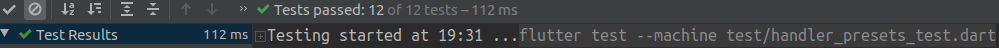
\includegraphics[scale = 0.5]{assets/t1.png}\\
        \caption[handler\_presets\_test.dart]{handler\_presets\_test.dart}
    \end{figure}
    \begin{figure}[H]
        \centering
        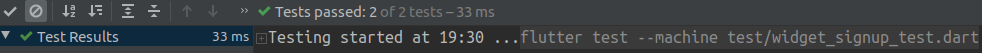
\includegraphics[scale = 0.5]{assets/t2.png}\\
        \caption[widget\_signup\_test.dart]{widget\_signup\_test.dart}
    \end{figure}
    \begin{figure}[H]
        \centering
        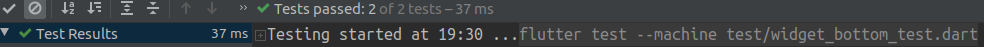
\includegraphics[scale = 0.5]{assets/t3.png}\\
        \caption[widget\_bottom\_test.dart]{widget\_bottom\_test.dart}
    \end{figure}
    \begin{figure}[H]
        \centering
        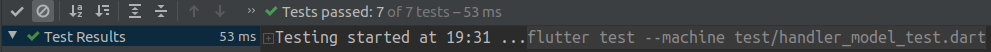
\includegraphics[scale = 0.5]{assets/t4.png}\\
        \caption[handler\_model\_test.dart]{handler\_model\_test.dart}
    \end{figure}
    \begin{figure}[H]
        \centering
        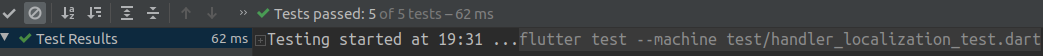
\includegraphics[scale = 0.45]{assets/t5.png}\\
        \caption[handler\_localization\_test.dart]{handler\_localization\_test.dart}
    \end{figure}
    \begin{figure}[H]
        \centering
        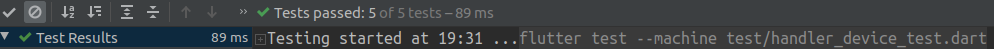
\includegraphics[scale = 0.5]{assets/t6.png}\\
        \caption[handler\_device\_test.dart]{handler\_device\_test.dart}
    \end{figure}
    \begin{figure}[H]
        \centering
        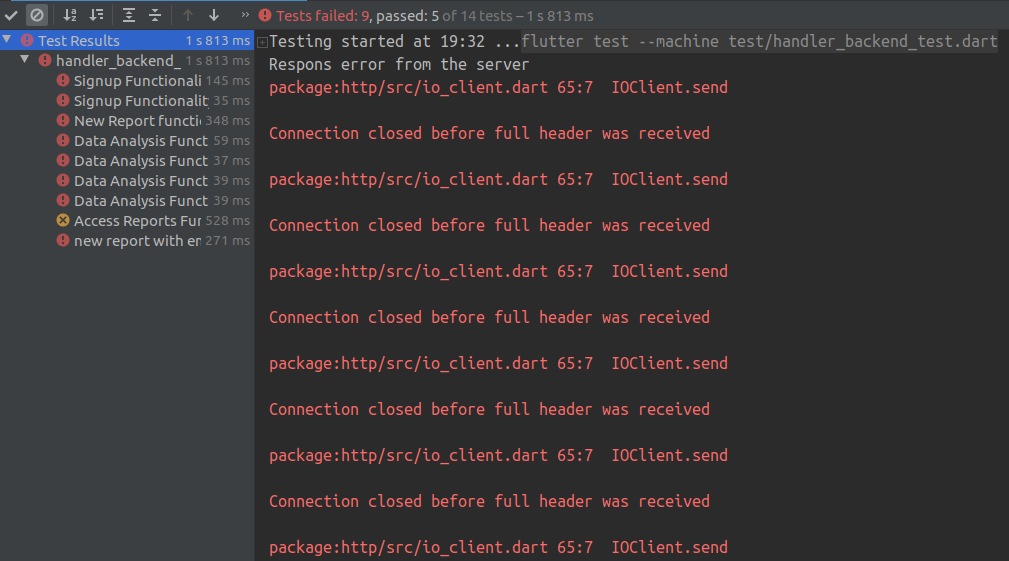
\includegraphics[scale = 0.5]{assets/t7.png}\\
        \caption[handler\_device\_test.dart]{handler\_backend\_test.dart}
    \end{figure}
    We tried to run a second time this, but here is the result:
    \begin{figure}[H]
        \centering
        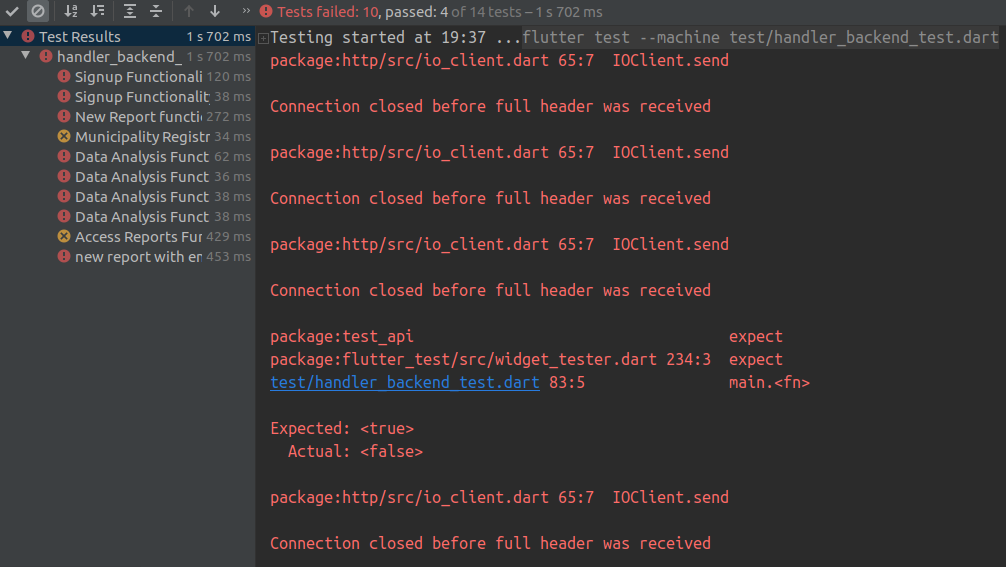
\includegraphics[scale = 0.5]{assets/t7v2.png}\\
        \caption[handler\_device\_test.dart 2]{handler\_device\_test.dart 2}
    \end{figure}


    \section{Document analysis}\label{sec:document-analysis}
    During the analysis of the documents (RASD, DD, ITD), we have found that there is no distinction between the functionalities offered by the app on the smartphone and the application on the web page.
    During the testing, we find out that on the smartphone is not allowed to register a user as a municipality.
    Moreover we noticed that on the web page is not possible to add a new report.


\end{document}